\documentclass{article}
\usepackage[utf8]{inputenc}
\usepackage{graphicx}
\usepackage[margin=1in]{geometry}

\title{Lab 3: Neuro - Measurement Station 2}
\author{Grego \& Peti}
\date{\today}

\begin{document}

\maketitle

\section*{Task 1: Series Resistor Measurement}

Rs = 2.17 kOhm (multimeter measurement), Rsmd nominal: 4.701 kOhm. Assembled circuit with Rs in series with Rsmd. Rsmd measured: 4.663 kOhm. Value close to nominal, circuit validated. Code and circuit functioning.

\subsection*{Visuals}
\begin{figure}[h!]
    \centering
    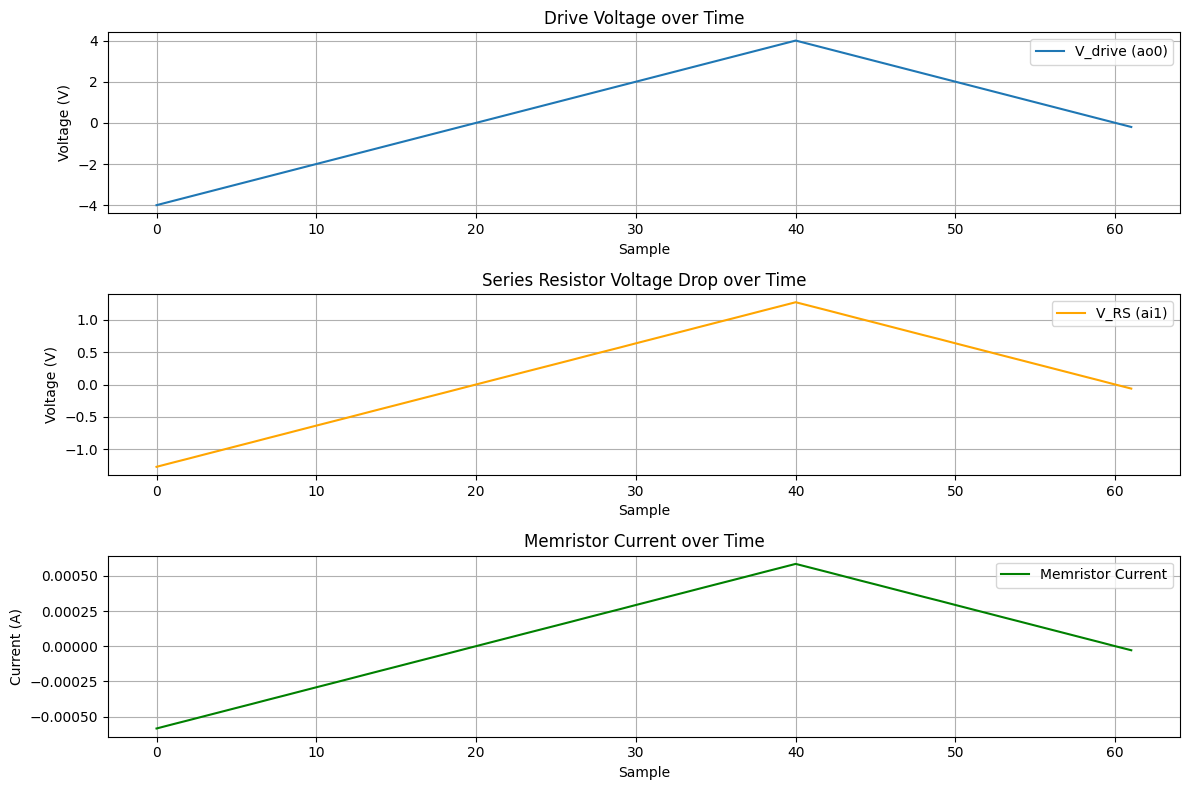
\includegraphics[width=0.8\textwidth]{task1_timeseries.png}
    \caption{Task 1: Time Series Plot}
    \label{fig:task1_timeseries}
\end{figure}

\begin{figure}[h!]
    \centering
    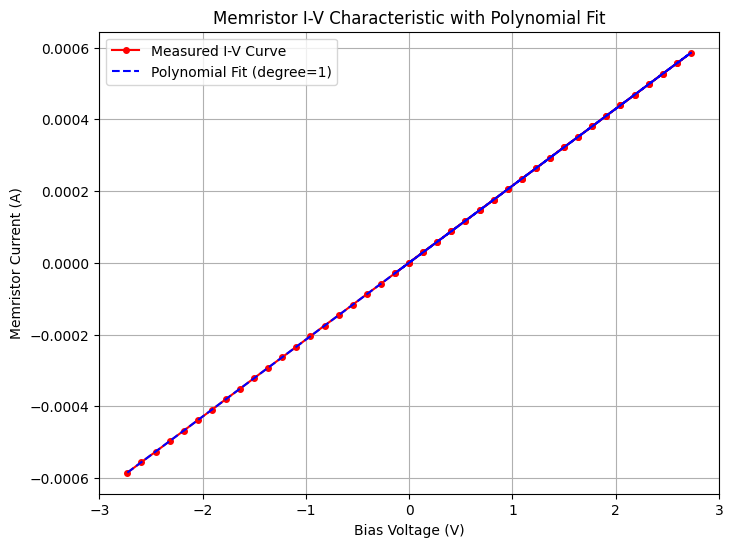
\includegraphics[width=0.8\textwidth]{task1_fit.png}
    \caption{Task 1: Fit Plot}
    \label{fig:task1_fit}
\end{figure}

\section*{Task 2: I(V) Curve Measurement}

Observed expected I(V) curve with characteristic jumps.

\subsection*{Visuals}
\begin{figure}[h!]
    \centering
    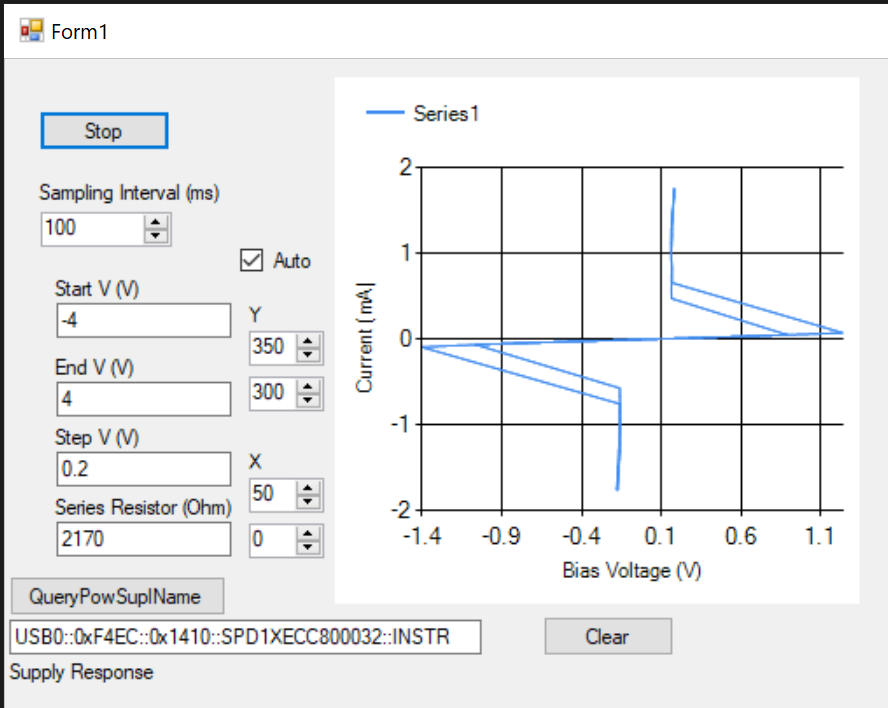
\includegraphics[width=0.8\textwidth]{task2_screenshot.png}
    \caption{Task 2: I(V) Curve Screenshot}
    \label{fig:task2_screenshot}
\end{figure}

\section*{Task 3: R(T) Characteristics Measurement Setup}

User interface, VISA/SCPI control, and data acquisition setup completed for R(T) measurements. Calculations for sample resistance and temperature implemented. Data logging and plotting updated. Power supply ON/OFF controls added. Remember to update the `PeltierPowerSupplyVisaResource`.

\end{document}
